\documentclass[a4paper, 11pt]{article}
\usepackage{amsmath}
\usepackage{amssymb}
\usepackage[czech]{babel}
\usepackage[utf8]{inputenc}
\usepackage[T1]{fontenc}
\usepackage{graphics}
\usepackage{graphicx}
\usepackage{multicol}
\usepackage{ulem}

\begin{document}
	\thispagestyle{empty}
	\title{VYSOKÉ UČENÍ TECHNICKÉ V BRNĚ \\ FAKULTA INFORMAČNÍCH TECHNOLOGIÍ}
	
	\date{}
	\maketitle
	\thispagestyle{empty}
	\begin{center}
	\huge{Matematická analýza}\\
	\Large{Domácí úkol 1 - varianta 7}
	
	\vspace{8cm}
	Hanák Karel - xhanak34\\
 	Chlupová Silvie - xchlup08\\
 	Krbálek Pavel - xkrbal02\\
 	Saranová Ivana - xsaran02\\	
 	Sedlák David - xsedla1d\\
 	\vspace{2cm}
	\textsc{16.3.2018}
	\end{center}	
	
	\newpage
	
	\setcounter{page}{1}
	 \section{Příklad}
	
	Rozložte následující funkci na parciální zlomky. Kořeny jmenovatele (které jsou celočíselné) najděte
	pomocí Hornerova schématu. Sestavte soustavu rovnic pro neurčité koeficienty; tuto soustavu můžete
	řešit pomocí vhodného softwaru. Napište výsledný tvar rozkladu. 
	
	\[f(x) = \frac{x^5-15x^2-55x-23}{x^5+7x^4+16x^3+16x^2+15x+9}\]
	
	
	\bigskip
	
	\section*{Postup řešení}
	
	1. Rovnice pro upravení Hornerovým schématem:
	\begin{equation}
	x^5+7x^4+16x^3+16x^2+15x+9 
	\end{equation}
	\begin{equation}
	p = 1; q = 9 
	\end{equation}
	\begin{equation}
	\text{kořeny: } d = \{\pm 1; \pm 3 ; \pm 9\}
	\end{equation}
	
	\bigskip
	
	2. Hornerovo schéma
	\begin{table}[h]
		\centering
		\begin{tabular}{rrrrrrr}
			& 1 & 7  & 16 & 16  & 15 & 9  \\
			-1 &   & -1 & -6 & -10 & -6 & -9 \\
			& 1 & 6  & 10 & 6   & 9  & 0 
		\end{tabular}
	\end{table}
	\begin{equation}
	(x+1)\cdot(x^4+6x^3+10x^2+6x+9)
	\end{equation}
	
	\begin{table}[h]
		\centering
		\begin{tabular}{rrrrrr}
			& 1 & 6  & 10 & 6  & 9  \\
			-3 &   & -3 & -9 & -3 & -9 \\
			& 1 & 3  & 1  & 3  & 0 
		\end{tabular}
	\end{table}
	\begin{equation}
	(x+1)\cdot(x+3)\cdot(x^3+3x^2+x+3)
	\end{equation}
	
	\begin{table}[h]
		\centering
		\begin{tabular}{rrrrrr}
			& 1 & 3  & 1 & 3  \\
			-3 &   & -3 & 0 & -3 \\
			& 1 & 0  & 1 & 0 
		\end{tabular}
	\end{table}
	\begin{equation}
	(x+1)\cdot(x+3)^2\cdot(x^2+1)
	\end{equation}
	
	\bigskip
	
	3. Nová rovnice po úpravě:
	\begin{equation}
	f(x) = \frac{x^5-15x^2-55x-23}{(x+1)\cdot(x+3)^2\cdot(x^2+1)}	
	\end{equation}
	
	\bigskip
	
	4. Rozložení na parciální zlomky (obecný tvar)
	\begin{equation}
	\frac{A}{x+1}+\frac{B}{x+3}+\frac{C}{(x+3)^2}+\frac{Dx+E}{x^2+1}
	\end{equation}
	\begin{equation}
	\begin{split}
	\frac{A\cdot(x+3)\cdot(x^2+1) + B\cdot(x+1)\cdot(x+3)\cdot(x^2+1)+}{(x+1)\cdot(x+3)^2\cdot(x^2+1)} \\
	\frac{+C\cdot(x+1)\cdot(x^2+1)+(Dx+E)\cdot(x+1)\cdot(x+3)^2}{(x+1)\cdot(x+3)^2\cdot(x^2+1)}
	\end{split}
	\end{equation}
	
	\bigskip
	
	5. Výpočet čitatelů obecného tvaru
	\begin{equation}
	\begin{gathered}
	x = -3 \\
	-20 = C\cdot(-2)\cdot10 \\
	\uuline{C = 1}
	\end{gathered}
	\end{equation}
	
	\begin{equation}
	\begin{gathered}
	x = -1 \\
	16 = A\cdot4\cdot2 \\
	\uuline{A = 2}
	\end{gathered}
	\end{equation}
	
	\begin{equation}
	\begin{gathered}
	x = 0 \\
	-23 = A\cdot9\cdot1 + B\cdot1\cdot3\cdot1 + C\cdot1\cdot1 + (E)\cdot1\cdot9 \\
	-23 = 18 + 3B + 1 + 9E \\
	-42 = 3B + 9E \\
	-14 = B + 3E
	\end{gathered}
	\end{equation}
	
	\begin{equation}
	\begin{gathered}
	x = 1 \\
	-92 = A\cdot16\cdot2 + B\cdot2\cdot4\cdot2 + C\cdot2\cdot2 + (D +E)\cdot2\cdot16 \\
	-92=64+16B+4+32D+32E \\
	-160=16B+32D+32E \\
	-10=B+2D+2E
	\end{gathered}
	\end{equation}
	
	\begin{equation}
	\begin{gathered}
	x = -2 \\
	19 = 2\cdot1\cdot5 + B\cdot(-1)\cdot1\cdot5 + (-2D+E)\cdot(-1)\cdot1 \\
	19 = 10 - 5B-5 + 2D -E \\
	14 = -5B +2D -E
	\end{gathered}
	\end{equation}
	
	\begin{equation}
	\begin{gathered}
	\text{Soustava rovnic řešená pomocí online softwaru} \\
	14 = -5B +2D -E \\
	-10=B+2D+2E \\
	-14 = B + 3E \\
	\uuline{B=-2} \\
	\uuline{D=0} \\
	\uuline{E=-4}
	\end{gathered}
	\end{equation}
	
	\bigskip
	
	Výsledek:
	\begin{equation}
	\uuline{f(x) = \frac{2}{x+1}-\frac{2}{x+3}+\frac{1}{(x+3)^2}-\frac{4}{x^2+1}}
	\end{equation}
	
 \section{Příklad}

Kužel má poloměr podstavy r a výšku v. Do tohoto kužele vepište jiný kužel tak, aby jeho vrchol ležel
 ve středu podstavy daného kužele a obvodová kružnice podstavy ležela v jeho stěně (kužel je „vzhůru
 nohama“). Zjistěte, kdy bude mít malý kužel maximální resp. minimální objem.

\section*{Postup řešení}
\begin{figure}[h!]
	\centering
	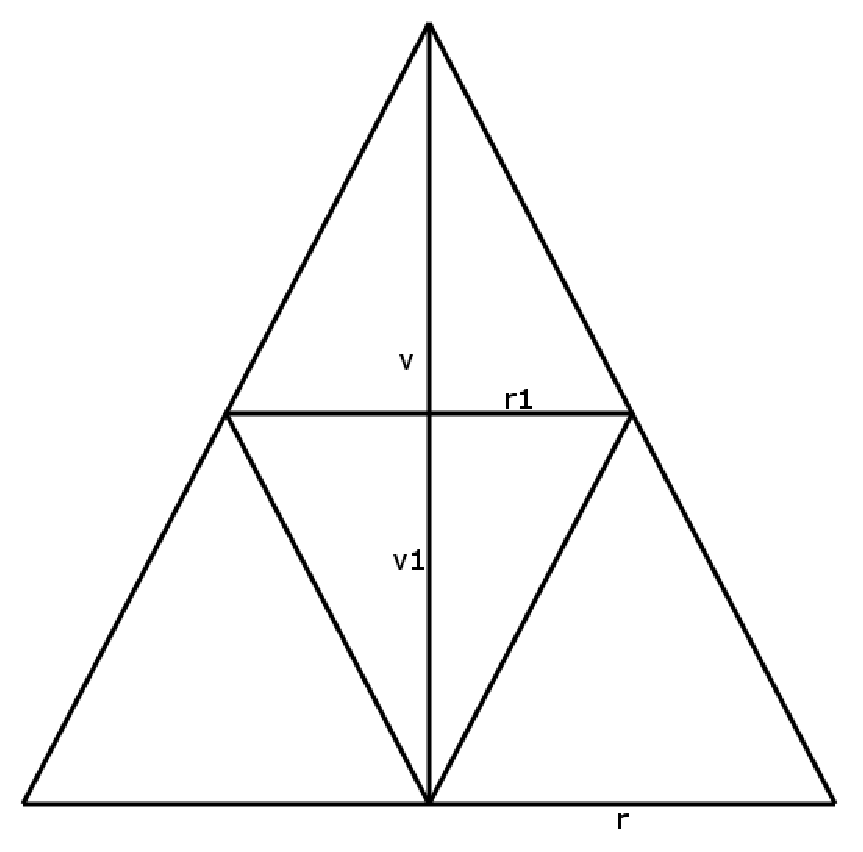
\includegraphics[width=0.55\linewidth]{image.eps}
	\caption{obr. k příkladu 2}
	\label{fig:image.eps}
\end{figure}

\begin{enumerate}
\item Na základě podobnosti troúhelníků vypočítáme vztah pro $v_1$
\begin{equation} 
\begin{gathered}
	\frac{v - v_1}{r_1} = \frac{v}{r} \\
	r \cdot v - r \cdot v_1 = r_1 \cdot v \\
	r \cdot v_1 = v \cdot (r - r_1)\\
	v_1 = \frac{v}{r}\cdot(r-r_1)\\
\end{gathered}
\end{equation}
\item Sestavíme účelovou funkci a určíme rozsah hodnot
\begin{equation} 
\begin{gathered}
V = \frac{1}{3} \cdot \pi \cdot {r_1}^2 \cdot v_1 \wedge v, r \in (0, \infty) \wedge v_1 \in (0, v) \wedge r_1 \in (0, r) \\
V = \frac{1}{3} \cdot \pi \cdot {r_1}^2 \cdot \frac{v}{r}\cdot(r-r_1) \\
V = \frac{1}{3} \cdot \pi \cdot {r_1}^2 \cdot \frac{v}{r}\cdot(r-r_1) \\
f(r_1) = \frac{1}{3} \cdot \pi \cdot \frac{v}{r}\cdot(r_1^2 \cdot r - r_1^3)\\
\end{gathered}
\end{equation}
\item Zderivujeme účelovou funkci
\begin{equation}f^\prime(r_1) = \frac{1}{3} \cdot \pi \cdot \frac{v}{r} \cdot (2 \cdot r \cdot r_1 - 3 \cdot {r_1}^2)\end{equation}
\item Zjistíme kdy je derivace rovna 0
\begin{equation} 
\begin{gathered}
\frac{1}{3} \cdot \pi \cdot \frac{v}{r} \cdot (2 \cdot r \cdot r_1 - 3 \cdot {r_1}^2) = 0\\
-3 \cdot r_1^2+2\cdot r \cdot r_1 = 0 \\
r_1 \cdot (-3\cdot r_1 + 2 \cdot r) = 0\\
r_1 \in \{0; \frac{2 \cdot r}{3}\}\\
\end{gathered}
\end{equation}
\item Lokální extrémy funkce mohou být v bodech, ve kterých je první derivace nulová, nebo neexistuje, první derivace naší účelové funkce je definovaná na celém intervalu (0, r) a jediný nulový bod na tomto intervalu je $r_1 = \frac{2\cdot r}{3}$, z první derivace také víme že před bodem $r_1 = \frac{2\cdot r}{3}$ funkční hodnota účelové funkce roste a po něm zase klesá, z toho je jasné že v tomto bodě bude účelová funkce dosahovat maxima na intervalu (0, r). Minima bude funkce dosahovat když se bude $r_1$ blížit hraničním bodům intervalu (0, r), hodnota minima se bude blížit k 0, přesnou hodnotu nelze určit, (v hraničních bodech by byla funkční hodnota nulová, ale ty nás nezajímají). 
\begin{equation}\uuline{f_{max} = f(\frac{2 \cdot r}{3}) = \frac{4 \cdot \pi \cdot r^2 \cdot v}{81}}\end{equation}
\end{enumerate}

\section{Příklad}
Nakreslete graf funkce $ f$, pro kterou platí: $ \mathcal{D}\textsubscript{$f$} = \mathbb{R}$ , je sudá, a pro $x \geq$ 0  platí:\\
v bodě $x = 1$ má nespojitost 2. druhu přičemž je spojitá zprava, \\
$f(0) = 2, f(1) = f(3) = 0, f(2) = 1$,\\
$f'(1) = 0, f'(2) = -2, \lim\limits_{x \to 0\textsuperscript{+}} f'(x) = 0, \lim\limits_{x \to 1\textsuperscript{+}} f'(x) = \infty$,\\
$f''(x) >$ 0 pro $x \in (0,1)$ a pro $x \in (3,\infty), f''(x)  <$ 0 pro $x \in (1,3)$,\\
přímka $y = -x$ je její asymptota.\\
Do obrázku nakreslete všechny asymptoty a tečny resp. polotečny v bodech, kde je zadaná derivace.

\begin{figure}[h!]
	\centering
	
\includegraphics[width=0.9\linewidth]{graph.eps}
	\caption{Graf funkce f}
	\label{fig:image}
\end{figure}
Naneštěstí funkci nelze nakreslit. Jeden problém je že $f''(x) >$ 0 pro $x \in (0,1)$, ale $f'(0) > f'(1)$.
\end{document}